\section{Topic models}

As our collective knowledge continues to be digitized and stored—in the 
form of news, blogs, web pages, scientific articles, books, images, sound,
video, and social networks—it becomes more difficult to find and discover 
what we are looking for. We need new computational tools to help organize, 
search and understand these vast amounts of information. To this end, machine learning provides topic models which are a suite of algorithms for discovering themes (or topics) that spread through a collection of documents.

In this section, we provide an overview of existing literature on topics models and then we describe two types of existing topic models: (i) the probabilistic model: Latent Dirichlet allocation and (ii) the non-probabilistic model: Non-negative Matrix Factorization.



\subsection{Literature review}

Topic modeling is gaining increasingly attention and is applied in a wide range of areas including on social networks such as Twitter and Facebook. From the view of methodology, topic models are separated into two groups: the non-probabilistic and probabilistic approaches. 


Most of probabilistic approaches are based on Latent Dirichlet Allocation (LDA) \cite{Blei}, which is the most popular standard tool in topic modeling. As a result, LDA has been used and extended in a variety of ways, and in particular 
for social networks and social media, so a great number of research papers that deal with LDA have been proposed.


Ramage et al. \cite{microblogs,Ramage} extended LDA to a supervised form and studied its application in
micro-blogging environment. More particularly, in \cite{Ramage} the Labeled LDA, a novel model of
multi-labeled corpora that directly addresses the credit assignment problem is introduced. In \cite{microblogs},
a scalable implementation of a partially supervised learning model (Labeled LDA) is proposed for 
discovering topics in microblogs like Twitter. This model maps the content of the Twitter feed 
into dimensions such as substance, style, status, and social characteristics of posts. Thus, this approach 
helps to efficiently characterize selected Twitter users along these learned dimensions and indicates that 
topic models can provide interpretable summaries of users’ tweet posts. Phan et al. \cite{Phan} studied the problem
of modeling short text through LDA. In particular, a general framework, based on LDA, for building classifiers 
with hidden topics discovered from large-scale data collections that can deal successfully with short and
sparse text \& Web segments. 

Moreover, Chang et al. \cite{chang} proposed a novel probabilistic topic model to analyze text corpora and 
infer descriptions of the entities and of relationships between those entities on Wikipedia. McCallum 
et al. \cite{McCallum} proposed a probabilistic generative model to simultaneously discover groups 
among the entities and topics among the corresponding text. Zhang et al. \cite{Zhang} introduced a model 
to incorporate LDA into a community detection process. More specifically, in this paper they designed a 
hierarchical Bayesian network based approach, namely GWNLDA(Generic-Weighted Network-LDA) which is inspired 
by LDA for discover probabilistic communities from complex networks. Similar work can be found in \cite{Liu} 
and \cite{Nallapati}.

Standard LDA is often less coherent when applied to microblog content like Twitter because tweets are short. 
To overcome this difficulty, some previous studies proposed to aggregate all the tweets of a user as a single
document. In \cite{Hong}, a topical classification of Twitter users and messages is provided. This paper 
deals with the problem of using topic models in microblogs by proposing schemes based on LDA 
and one extended model based on the Author-Topic model. It also presents that topic models aims 
some classification problems by indicating that topic models learned from aggregated messages
by the same user obtaining higher accuracy. Also, a different approach on topic modeling of Tweets is provided
in \cite{improving}. This paper focus on how to improve clustering metrics and topic coherence with existing algorithms. More specifically, it provides two novel schemes that lead to significantly improved LDA topic models on Twitter content without requiring any modification of the underlying LDA machinery. The first one is about pooling tweets by hashtags that yields a great improvement in all metrics for topic coherence across three diverse Twitter datasets, and the second is an automatic hashtag assignment scheme further improves the hashtag pooling results on a subset of metrics.


Non-probabilistic topic models are also very popular. One of the most known representative model is the Non-Negative Matrix Factorization (NMF) \cite{paa94,lee99}. Yan et.al \cite{Yan},  proposed a novel term weight called Ncut-weighted, which measures term’s discriminability according to the words cooccurrences, for short text clustering. More particularly, the experiments show that the clustering performance of NMF is greatly improved with terms weighted by the Ncut-weight. Due to the severe sparsity of short texts, in\cite{yan2013learning}, a different approach on the non-negative matrix factorization is introduced. This approach first learns topics from term correlation data using symmetric non-negative matrix factorization, and then infers the topics of documents. The experimental results on three short text data sets show that this method provides substantially better performance than other baseline methods like LDA.



\subsection{Latent dirichlet allocation}


The idea behind Latent Dirichlet allocation (LDA) \cite{Blei, heinrich2005parameter, steyvers}, which is an unsupervised machine learning technique, is to model documents as arising from multiple topics, where a topic
is defined to be a distribution over a fixed vocabulary of terms. Specifically, we assume that K topics are
associated with a collection, and that each document exhibits these topics with different proportions. 
The interaction between the observed documents and hidden topic structure is manifest in the probabilistic generative process associated with LDA. This generative process is as follows:

To generate a document:
\begin{enumerate}
\item Randomly choose a distribution over topics.
\item For each word in the document
\begin{enumerate}
\item Randomly choose a topic from the distribution over topics in step \#1.
\item Randomly choose a word from the corresponding distribution over the vocabulary
\end{enumerate}
\end{enumerate}

So, this statistical model reflects the intuition that documents exhibit multiple topics. 
Each document exhibits the topics with different proportion (step \#1); each word in each document is drawn from one of the topics (step \#2b), where the selected topic is chosen 
from the per-document distribution over topics (step \#2a).

\begin{figure}
  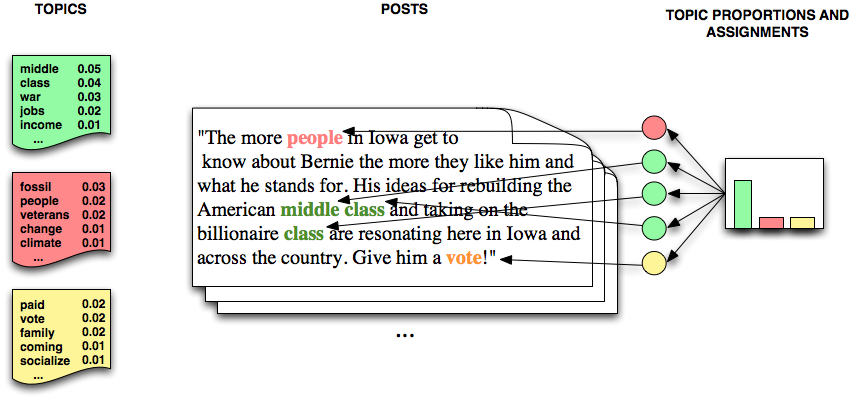
\includegraphics[width=\linewidth]{lda}
  \caption{An LDA example.}
  \label{fig:lda}
\end{figure}

In Figure \ref{fig:lda}, an LDA example is illustrated. We assume that we have three topics, which are distributions over words, exist for the whole collection (far left). Each document is assumed to be generated as follows. First choose a distribution over the topics (the histogram at right) and then, for each word, choose a topic assignment (the colored coins) and choose the 
word from the corresponding topic. As we can see, in this example the particular document is assigned to the first topic with higher probability compare to the others.

\subsection{Non-negative Matrix Factorization}

Non-negative matrix factorization (NMF) is an unsupervised family of algorithms from linear algebra that simultaneously perform dimension reduction and clustering. NMF was first introduced by Paatero and Tapper \cite{paa94} as positive matrix factorization and subsequently
popularized by Lee and Seung \cite{lee99}.

In Figure \ref{fig:nmf}, NMF takes a non-negative matrix \textbf{A} as an input, and factorizes it into two smaller non-negative matrices \textbf{W} and \textbf{H}, each having \textit{k} dimensions. When multiplied together, these factors approximate the original matrix \textbf{A}. The specified parameter \textit{k} controls the number of topics that will be produced. The rows of the matrix \textbf{W} provides weights that indicate the strength of association between documents and topics. The columns of the \textbf{H} that indicate the strength of association between terms and topics. By ordering the values in a given column and selecting the top-ranked terms, we can produce a description of the corresponding topic.

\begin{figure}
  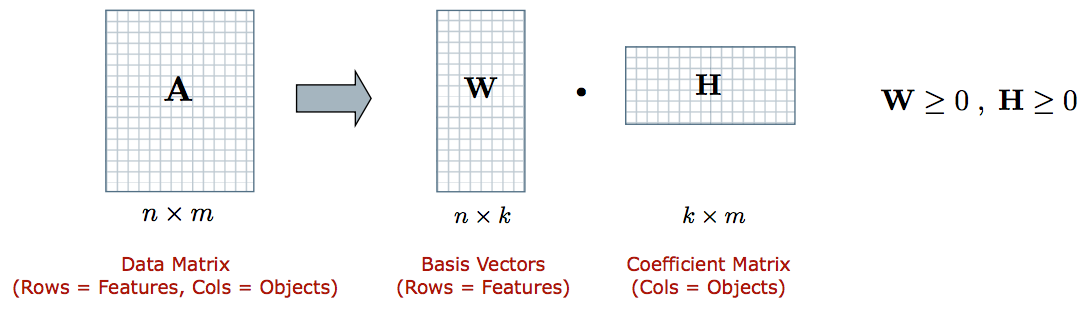
\includegraphics[width=\linewidth]{nmf}
  \caption{Illustration of approximate non-negative matrix factorization: the matrix A is represented by the two smaller matrices W and H, which, when multiplied, approximately reconstruct A}
  \label{fig:nmf}
\end{figure}
